\chapter{Stand der Technik}

In diesem Kapitel werden die aktuelle technische Lösungen im Bereich Cloud Computing und verteiltes Rechnen vorgestellt, sowie die gängigsten Softwarewerkzeuge mit denen diese Systeme erzeugt und verwaltet werden können.

\section{Cloud Computing}
Cloud Computing besitzt in der Literatur mehrere Definitionen.\cite{Marston2011} Die am weitesten verbreitete Definition wurde vom National Institute of Standards and Technology (NIST) festgelegt.Nach dieser Definition ist Cloud Computing ein Modell, das einen allgegenwärtigen, bequemen, bedarfsgerechten Zugang zu einem gemeinsamen Pool an konfigurierbarer Rechenressourcen die jederzeit und von jedem Ort aus über das Internet oder ein Netzwerk schnell zur Verfügung gestellt 
werden können. Es wird durch fünf Eigenschaften charakterisiert:   \\
\begin{itemize}
	\item On-Demand und Selbstbedienung: Kunden können die Rechenressourcen selbständig nach Bedarf ohne menschliche Interaktion anfordern
	\item Breiter Netzzugang: Ressourcen sind über Netzwerkverbindung erreichbar über standardisierte Zugriffsmechanismen
	\item Ressourcen-Pooling: Die Ressourcen des Anbieters werden aus mehreren physikalischen Recheneinheiten zusammengelegt, die auch geographisch nicht an einem Ort sein müssen. Mit einem Multi-Tenant Modell werden die Ressourcen dynamisch je nach Kundenbedarf zugewiesen. Der Kunde hat keinen Kenntnis oder Kontrolle über den genauen Standort der bereitgestellten Ressourcen.
	\item Schnelle Elastizität: Bereitgestellte Ressourcen können flexibel bereitgestellt und freigegeben werden. Für den Kunden erscheint die Menge der bereitgestellten Ressourcen unbegrenzt, sie können jederzeit in beliebiger Menge gebucht werden.
	\item Measured Service: Nutzung der Cloud Systeme wird automatisch gemessen und optimiert anhand einer Messfunktion, die nach Metriken wie Speicher, Verarbeitung, Bandbreite und Benutzerknoten die Ressourcennutzung ermittelt. Kosten für den Cloud Dienst werden nach der gemessenen Nutzung ermittelt (Pay per Use) \cite{Mell2011}
\end{itemize}

Cloud Computing ist ein Geschäftsmodell für die Bereitstellung von IT Infrastruktur, Komponenten und Anwendungen, welches mittlerweile den Markt dominiert. \cite{Benlian2018} Cloud Service Anbieter betreiben die IT Infrastruktur und stellen sie für Kunden zur Verfügung. Kunden müssen nicht ihre eigene Infrastruktur aufbauen, sie können die benötigten Kapazitäten je nach aktueller Bedarf einkaufen. Diese Lösung ermöglicht den Kunden hohe Rechenkapazitäten zu erhalten, die diese selber nicht aufbauen und betreiben können.\cite{Arasaratnam2011} Der Markt für Cloud Infrastruktur ist ein weiterhin wachsender Markt (Stand Q4 2023) mit 270 Milliarden US Dollar Gesamtausgaben für das Jahr 2023. Die größten Cloud Service Anbieter und deren Marktanteil ist in der Tabelle \ref{cloud_marktanteile} aufgelistet.

\begin{table}
	\centering
		\caption{Cloud Anbieter und deren Marktanteile in Q4 2023} 
		\label{cloud_marktanteile}
		\begin{tabular}{|c | c|} 
			\hline
			Anbieter & Marktanteil in Prozent \\
			\hline\hline
			AWS & 31\%\\ 
			\hline
			Azure & 24\% \\
			\hline
			Google Cloud & 11\% \\
			\hline
			Alibaba Cloud & 4\% \\
			\hline
			salesforce & 3\% \\
			\hline
			IBM Cloud & 2\% \\ 
			\hline
			ORACLE & 2\% \\ 
			\hline
			Tencent Cloud & 2\% \\ 
			\hline
		\end{tabular}
\end{table}

Cloud Computing bietet verschiedene Geschäftsmodelle für Kunden an, die je nach Kundenbedarf fertigen Softwareplattform oder reine Rechenressourcen für eigene Applikationen bereitstellen:

\begin{itemize}
	\item Infrastructure as a Service (IaaS): Kunde kauft Rechenressourcen nach Bedarf ein, Cloud Anbieter stellt eine \gls{virtuelle Maschine} dem Kunden zur Verfügung. Kunde kann über eine API auf die gemietete Infrastruktur zugreifen. Er kann Komponenten wie Betriebssystem, Applikationen und Laufzeitumgebung selber verwalten. Cloud Anbieter ist für die Bereitstellung der Rechenressourcen wie Rechenleistung, Speicher, Netzwerk sowie jegliche Hardwareausfälle verantwortlich.
	\item Platform as a Service (PaaS): Kunde lässt eine eigene Applikation auf der Cloud Infrastruktur ausführen. Cloud Anbieter übernimmt die Bereitstellung der Hardware und Ressourcen wie bei IaaS, zusätzlich aber auch das Betriebssystem und Laufzeitumgebung. So kann der Kunde seine Daten und Applikationen direkt in die gemietete Cloud Umgebung platzieren ohne weitere Aufwände.
	\item Software as a Service (SaaS): Cloud Anbieter bietet online Applikationen an Kunden an. Der Anbieter stellt dabei die benötigte IT Infrastruktur bereit, inklusive Einrichtung der Laufzeitumgebung und Bereitstellung der Rechenressourcen (IaaS und PaaS). Kunde benutzt die bereitgestellte Applikationen über definierte Benutzeroberfläche, meistens wird eine über Web Browser erreichbare Web Benutzeroberfläche angeboten. Der Kunde ist in diesem Modell der Endbenutzer der vom Cloud Anbieter gestellten Applikation.

\end{itemize} \cite{Mell2011}

Die Zuständigkeiten zwischen Cloud Anbieter und Kunde des Cloud Dienstes für die verschiedenen Geschäftsmodelle ist in der Abbildung \ref{cloud_modelle} dargestellt. Hier ist es gut erkennbar wie die Zuständigkeiten von IaaS zu Saas hin immer mehr Richtung Cloud Anbieter verlagert werden.

\begin{figure}[htbp]
	\centering
	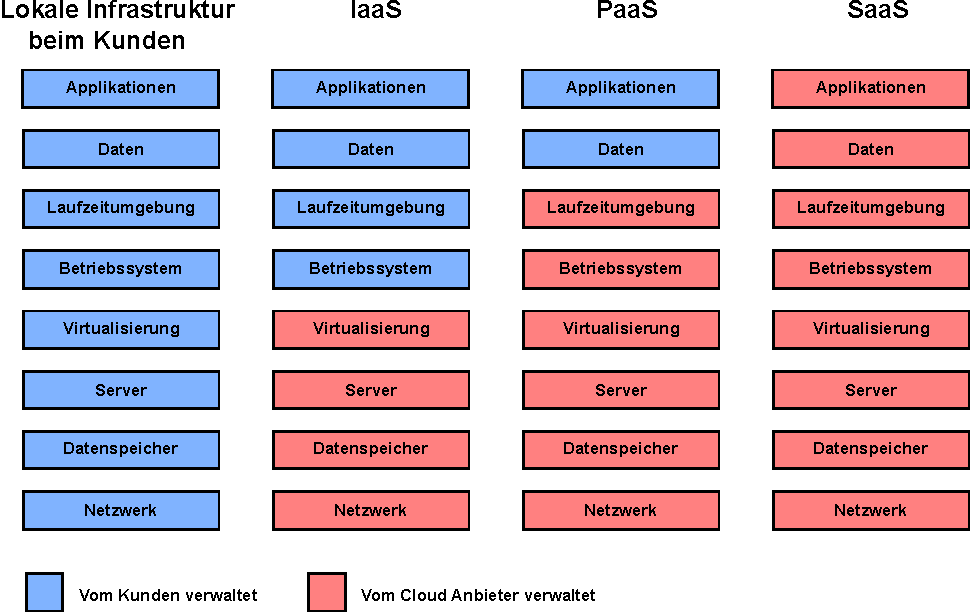
\includegraphics[width=\textwidth]{./content/graphics/cloud_models.pdf}
	\caption{Vergleich der Zuständigkeiten zwischen Cloud Anbieter und Kunden bei verschiedenen Geschäftsmodellen}
	\label{cloud_modelle}
\end{figure}

In der heutigen Zeit sind viele im Alltag verbreitete Applikationen als Cloud Service ausgelegt. Datenspeicherung (Dropbox, Google Drive), Dokumente bearbeiten (Office 365, Google Docs), Business-management (SAP ByDesign) und Videospiele (Geforce Now) sind typische Anwendungsbereiche hierfür. 

\section{Distributed Computing}

Distributed Computing bezeichnet verteilte Systeme, die aus dem Zusammenschluss von mehreren physikalischen Recheneinheiten bestehen. Auf dieser Weise können sie an einem gemeinsamen Problem arbeiten. Hierdurch ist es möglich auch große Datenmengen oder komplexe Rechenaufgaben effizienter zu verarbeiten als mit einzelnen Recheneinheiten. \cite{AWS2023} Die einzelnen Recheneinheiten in einem Verteilten System werden als Nodes genannt. \cite{ord1994scale} Verteilte Systeme sind heutzutage Stand der Technik, da die Rechenleistung von einzelnen Rechenkernen nicht beliebig skalierbar ist. Wenn also hohe Rechenleistung benötigt wird, kann dies  durch die Zusammenschaltung von mehreren Recheneinheiten und die Parallelisierung von Rechenaufgaben erfolgen, die den Ansatz der Distributed Computing verfolgt. Verteiltes Rechnen bildet die Grundlage für Cloud Computing, da die dafür benötigten Ressourcen mit einzelnen physikalischen Rechnern nicht realisierbar sind. Heutzutage verbreitete Cloud Dienste Provider (Google, Facebook) verwenden verteilte Systeme für ihre Infrastruktur. \cite{arpaci2018operating} 

\section{Edge Computing}

Edge Computing ist eine Form von Distributed Computing. In diesem Kontext werden die Endgeräte, wo Daten entstehen oder benötigt werden als Edge bezeichnet. Durch die zunehmende Digitalisierung der Stadt Infrastruktur und alltägliche Gegenstände wie Mobiltelefone, Uhren, Hausgegenstände entstehen immer höhere Datenmengen, die verarbeitet werden müssen. Im Cloud Computing Ansatz werden die Daten in geographisch weit entfernten Cloud Servern verarbeitet und wieder an die Endgeräte auf der Edge Ebene zurückgesendet. Hierdurch erhöht sich die Latenz sowie die insgesamt benötigte Netzwerkbandbreite. Edge Computing verlagert die Datenverarbeitung in die Nähe der Geräte, wo die Daten entstehen und die verarbeiteten Daten benötigt werden, also in die Edge Ebene und reduziert damit die Latenz und die benötigte Gesamtbandbreite zu entfernten Cloud Servern. \cite{Wang2019} Motiviert wird diese Entwicklung dadurch, dass Netzwerkbandbreite sich deutlich langsamer entwickelt als die Zunahme an erzeuge Datenmengen.\cite{Shi2016} Latenzreduzierung ist relevant für Echtzeitsysteme wie Datenauswertung für autonome Fahrzeuge, aber auch für Anwendungen, wo Berührungsrückmeldungen an dem Benutzer zurückgemeldet werden sollen. Damit der Mensch keinen Latenz empfindet, muss die Kommunikation und Datenverarbeitung innerhalb von 1 ms erfolgen. \cite{Varsha2017} Edge Computing ist eine Alternative für lokale Berechnungen auf dem jeweiligen Endgerät. Diese Endgeräte haben in vielen Fällen nur begrenzte Rechenleistung, so dass die lokale Datenverarbeitung nicht sinnvoll umsetzbar ist. Rechenoperationen können auch in Cloud Systeme ausgelagert werden, allerdings resultiert dieser Ansatz in höhere Latenzen und Bandbreitenauslastungen. \cite{Lin2020} 

\section{Applikationsmanagement in Cloud Systemen}

Applikationen haben in den meisten Fällen Abhängigkeiten zu weiteren Softwarekomponenten, die auf dem ausführenden Betriebssystem installiert werden muss. Das Betriebssystem und die darauf installierte Softwarekomponenten nennt man Laufzeitumgebung. Verschiedene Applikationen können verschiedene Versionen von zusätzlichen Softwarekomponenten nutzen, so dass sie nicht gleichzeitig auf dem selben Betriebssystem und Laufzeitumgebung ausführbar sind. In traditionellen Architekturen wird deswegen eine begrenzte Anzahl an Applikationen mit kompatibler Laufzeitumgebung auf einer physikalischen Maschine ausgeführt, die in eine nicht optimale Auslastung der Hardwareressourcen resultiert. Um die Auslastung zu optimieren, wurde das Konzept der Virtualisierung entwickelt. Die physische Ressourcen werden in mehrere virtuelle Ressourcen aufgeteilt. Hierdurch ist es möglich auf einer physikalischen Maschine mehrere voneinander unabhängige Laufzeitumgebungen einzurichten. Virtualisierung wurde bereits in den 1960-er Jahren entwickelt, allerdings wurde dafür spezielle Hardware benötigt. Für die aktuell verbreitete x86-er Architektur wurde die Virtualisierung von VMWare in 1999 umgesetzt. \cite{Bugnion2012} In der Informationstechnik haben sich zwei Virtualisierungsmethoden durchgesetzt, die in den folgenden Abschnitten vorgestellt werden. Ein Überblick über die Struktur der beiden Methoden im Vergleich zu einem klassischen System ohne Virtualisierung ist in der Abbildung \ref{virtualisierung_optionen} dargestellt. 

\begin{figure}[htbp]
	\centering
	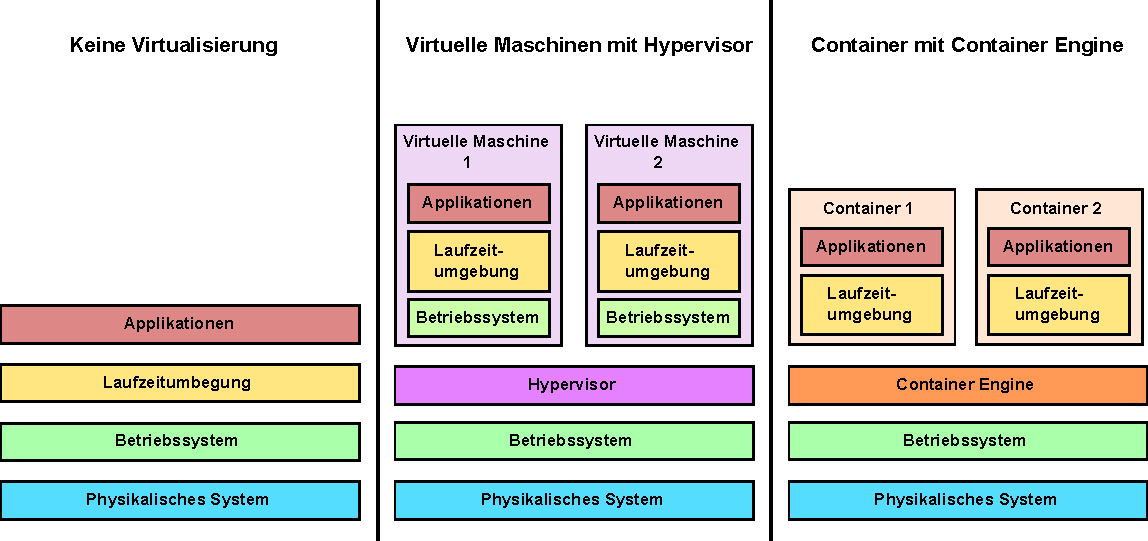
\includegraphics[width=\textwidth]{./content/graphics/applikation_management.pdf}
	\caption{Vergleich keine Virtualisierung zu den beiden verwendeten Virtualisierungsansätzen}
	\label{virtualisierung_optionen}
\end{figure}

\subsection{Virtuelle Maschine}

In Cloud Systemen wurden in den letzten Jahrzehnten hauptsächlich virtuelle Maschinen als Virtualisierungsumgebung verwendet. Bei dieser Methode wird ein neues virtuelles System mit eigenem Betriebssystem erzeugt. Diese neue Umgebungen werden Virtuelle Maschinen bezeichnet. \cite{Pahl2015} Technisch umgesetzt wird das Konzept indem physikalischer Hardware per Software emuliert wird. Erstellt und verwaltet werden die virtuelle Maschinen durch eine Softwarekomponente namens Hypervisor. Der Hypervisor ist die Softwareschicht zwischen der physikalischen Hardware und virtuelle Maschinen. Es implementiert die folgenden Funktionalitäten die nötig sind um eine virtuelle Maschine zu erstellen:
\begin{itemize}
	\item CPU Virtualisierung: der Hypervisor präsentiert eine virtuelle CPU (vCPU) in der virtuellen Maschine. Diese CPU funktioniert wie eine echte physikalische CPU innerhalb der virtuellen Maschine. Anweisungen, die Hardwarezugriff benötigen würden, werden vom Hypervisor verarbeitet. Der Hypervisor kann die verfügbaren CPU Ressourcen dynamisch je nach Bedarf an die virtuellen Maschinen zur Verfügung stellen aber auch die maximale CPU Nutzung von den Maschinen begrenzen bei Bedarf. 
	\item Speichervirtualisierung: Für die virtuelle Maschinen werden virtuelle Speicherbereiche erzeugt. Der Hypervisor ordnet diese virtuelle Speicherbereiche an physikalisch vorhandene Speicherbereiche zu. Der Hypervisor kann den maximal verfügbaren Speicher der virtuellen Maschinen einschränken um deren Ressourcennutzung zu beschränken.
	\item Virtualisierung von Ein/Ausgabegeräten: Damit virtuelle Maschinen die physikalisch vorhandene Ein- und Ausgabekomponenten wie Netzwerkadapter nutzen können, werden virtuelle Komponenten des selben Typs in der virtuellen Maschine erstellt, die mit den physikalisch vorhandenen Komponenten verknüpft werden. Hierbei können auch mehrere virtuelle Maschinen eine Komponente teilen. Zusätzlich können durch Regeln die Zugriffsrechte der virtuellen Maschinen eingeschränkt werden.  \cite{Dall2014}
\end{itemize}
 Dieser Ansatz ermöglicht auch die Verwendung von verschiedenen Betriebssystemen in verschiedene virtuelle Maschinen die auf dem selben physikalischen System laufen und bietet damit eine hohe Flexibilität bei den bereitgestellten Laufzeitumgebung für die jeweiligen Applikationen die in der Umgebung ausgeführt werden. Die schematische Darstellung eines Systems mit mehreren virtuellen Maschinen ist in der Abbildung \ref{virtualisierung_optionen} in der mittleren Spalte dargestellt. Applikationen in virtuelle Maschinen auszuführen hat gegenüber keine Virtualisierung auch Nachteile. Hauptnachteil der virtuellen Maschinen ist die zusätzliche Ressourcenaufwand. Für jede unterschiedliche Instanz einer virtuellen Maschine muss ein zusätzliches Betriebssystem mit entsprechenden Laufzeitumgebung zusätzlich zu der auszuführenden Applikation vorhanden sein. Hierdurch ergibt sich eine deutlich höhere Festplattenspeicher und Arbeitsspeicher Auslastung. Ebenfalls wird für das Ausführen des Betriebssystems und virtuelle Hardwarekomponenten in der virtuellen Maschine zusätzliche Rechenleistung benötigt. \cite{Mavridis2019} 

\subsection{Container}

Um die vorhin genannte Nachteile der virtuellen Maschinen zu umgehen, haben sich Container als alternative Methode für Virtualisierung in den letzten Jahren verbreitet. Containerisierung ist eine Virtualisierungsmethode, die im Gegensatz zu virtuellen Maschinen keine neue Betriebssysteme für neue virtuelle Umgebungen ausführt. Applikationen werden direkt auf dem Betriebssystem des physikalischen Systems ausgeführt.  Hierdurch sind Container kleiner, da sie kein Betriebssystem zusätzlich enthalten müssen im Vergleich zu virtuelle Maschinen. Container sind durch das Wegfallen des zusätzlichen Betriebssystems auch effizienter im Bezug auf Rechenressourcen. Zusätzlich können Container auch deutlich schneller gestartet werden da kein Betriebssystem beim Startvorgang gebootet werden muss (etwa 50ms bei Container, 30-40s bei virtuelle Maschinen). \cite{Martin2018} Ähnlich wie virtuelle Maschinen auf einem System durch den Hypervisor verwaltet werden, werden Container mit einem Container Runtime Softwaremodul verwaltet. Die Isolierung erfolgt bei Container nicht durch virtuelle Hardwarekomponenten sondern auf Betriebssystemebene. Container nutzen die Möglichkeiten des Linux Kernels Applikationen voneinander zu isolieren. Dies wird durch sogenannte namespaces ermöglicht. Namespaces können eine bestimmte globale Ressource für ein Prozess isolieren, so dass es wie eine eigene Instanz erscheint. Folgende namespaces sind im Linux Kernel verfügbar:
\begin{itemize}
	\item Mount Namespace: Isoliert das Dateisystem im Container. Die Prozesse im Container können nur die Pfade im Dateisystem sehen und darauf zugreifen die explizit per mount() Funktion zum jeweiligen Namespace hinzugefügt wurden.
	\item UTS Namespace: Isoliert die Prozessidentifikatoren für den Container. Prozessnamen und Domänenamen können dadurch beliebig umbenannt werden. Dies ist nützlich wenn in Prozessen Aufstartskripte verwendet werden, die bestimmte Prozessnamen voraussetzen.
	\item IPC Namespace: Isoliert die zwischen-Prozess Kommunikation (Inter Process Communication) Ressourcen im Container. Hierdurch können Container die verschiedene IPC namespaces zugehören Ressourcen für zwischen-Prozess Kommunikation wie Semaphoren oder Shared Memory mit gleichen Namen anlegen, ohne dass sie miteinander kommunizieren können.
	\item PID Namespace: Prozesse im Container haben eigene Prozessidentifikationsnummern (PID). Somit kann in jedem Container ein Initialisierungsprozess mit PID 1 vorkommen. Ein weiterer Effekt der PID Isolierung ist, dass jeder Container einen eigenen /proc Ordner erhält, das <bedeutet dass Container nur ihre eigene Prozesse einsehen können, die restlichen Prozesse im System sind von innerhalb des Containers unsichtbar. Das System selbst kann die Containerprozesse sehen, allerdings haben diese Containerprozesse aus Systemsicht andere PIDs als innerhalb des Containers.
	\item Network Namespace: Isoliert Netzwerkressourcen für die Container. Dies beinhaltet Netzwerkadapter, Firewall und Routingtabellen. Die Netzwerkkonfiguration kann in jedem Container unterschiedlich angepasst werden, es ist möglich verschiedene virtuelle oder physikalische Netzwerkadapter zum Container hinzuzufügen. Die konfigurierbare Routingtabelle pro Container ermöglicht einen konfigurierbaren Maß an Netzwerkisolation.
\end{itemize} 

Namespaces decken den Bedarf an Prozess und Laufzeitumgebungsisolation für die Virtualisierung ab. Eine weitere Anforderung ist die Begrenzung von verfügbaren Ressourcen für die jeweiligen virtuellen Umgebungen. Um dies zu ermöglichen bietet Linux ebenfalls im Kernel eine Möglichkeit an. Cgroups ermöglichen die Gruppierung von Prozessen um deren Ressourcen zu verwalten. Es kann die CPU Zeit, Speicherverbrauch und Netzwerkbandbreite für die Gruppen eingeschränkt werden. Bei der Virtualisierung mit Container bekommt jeder Container eine eigene cgroup, so dass deren Ressourcenverbrauch durch den Container Runtime eingeschränkt werden kann. \cite{Red_2024} 
Die systematische Darstellung eines Systems mit Container als Virtualisierungsmethode ist in der Abbildung \ref{virtualisierung_optionen} in der rechten Spalte dargestellt. 

\section{Orchestrierung von virtuellen Umgebungen}

Softwarekomponenten wie Hypervisor und Container Runtime verwalten die virtuellen Umgebungen auf einer physikalischen Maschine. Sie eignen sich also dazu, Rechenressourcen lokal flexibel zu verwalten und bilden damit die Grundlage für Cloud Computing Systeme. Cloud Systeme bestehen allerdings aus viele physikalische Maschinen, die oft auch örtlich verteilt sind. Für diese Systeme wäre es sehr aufwändig, die virtuellen Umgebungen auf den einzelnen physikalischen Maschinen manuell zu verwalten, aus diesem Grund werden Programme für die Orchestrierung verwendet, die die Verwaltung von den virtuellen Umgebungen auf verschiedenen physikalischen Systemen automatisieren. 

\subsection{Virtuelle Maschine Orchestrierung}

Cloud Systeme werden mit CLoud System Management Plattforme verwaltet. Diese sind in der Regel modular aufgebaut und bieten diverse Module für die Einrichtung, Verwaltung und Überwachung von Cloud Systemen an. Virtuelle Maschinen sind in Cloud Systemen weiterhin stark verbreitet. Aus diesem Grund bieten diese Management Plattforme auch entsprechende Hypervisor und Orchestrierer Module an. 

Für die beispielhafte Vorstellung eines solchen Management Platforms wird die Architektur des Open Source Plattforms OpenStack genommen. Es verfolgt ebenfalls eine modulare Struktur, wo verschiedene Module, die Services genannt werden verschiedene Aufgaben übernehmen. Eine schematische Darstellung der Kernkomponenten kann in der Abbildung \ref{openstack_arch} betrachtet werden. Im folgenden Abschnitt wird die Funktion der einzelnen Module kurz erklärt:

\begin{figure}[htbp]
	\centering
	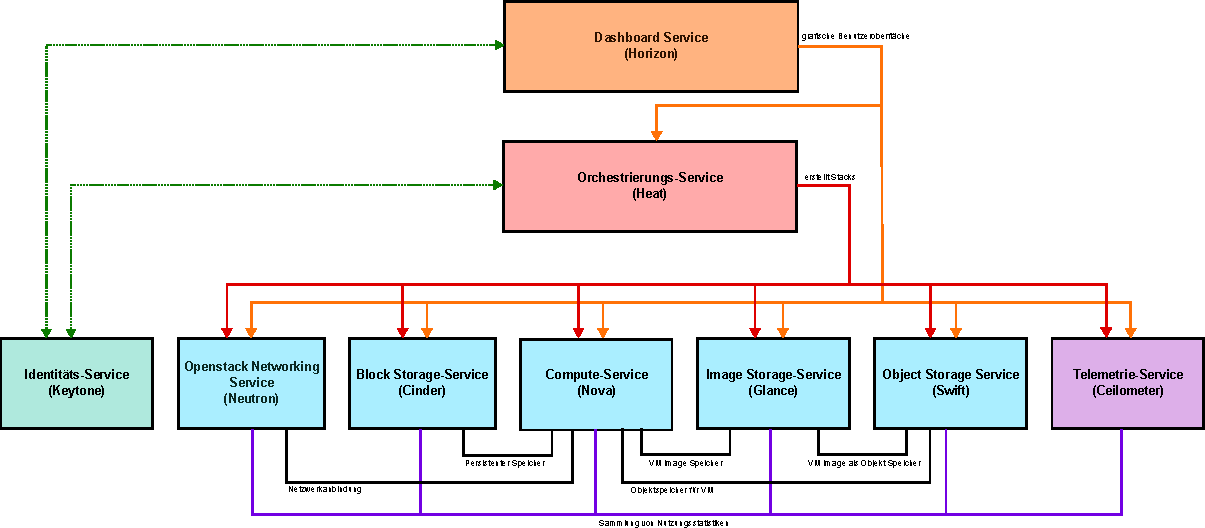
\includegraphics[width=\textwidth]{./content/graphics/openstack_arch.pdf}
	\caption{Schematische Darstellung der OpenStack Architektur}
	\label{openstack_arch}
\end{figure}

\begin{itemize}
	\item Dashboard (Horizon): Stellt eine grafische Benutzeroberfläche zur Verfügung, die über Wer Browser erreichbar ist. Mit diese Oberfläche können Benutzer und Administratoren neue Virtuelle Umgebungen erstellen, Netzwerkeinstellungen und Zugriffe verwalten. 
	\item Orchestrierer (Heat): Der Orchestrierer stellt Vorlagen zur Verfügung für die Erstellung und Verwaltung von CLoud Ressourcen. Mit Hilfe diese Vorlagen können sogenannte \enquote{Stacks} erstellt werden, die eine Sammlung an Ressourcen sind. In diesem Fall können diese Ressourcen beispielweise Hypervisoren, Virtualisierungs-Engines, Container-Engines, Management-Services, Container-Orchestrierung, Benutzeroberflächen beinhalten. 
	\item Identity (Keystone): Stellt Authentifizierung und Authorisierung für Benutzer zur Verfügung. Unterstützt verschiedene Methoden für Authentifizierung, wie Benutzername und Passwort, Token oder Amazon Web Services log-in.
	\item Networking (Neutron): Erstellt und verwaltet das virtuelle Netzwerkinfrastruktur im Cloud System. 
	\item Block Storage: Block Storage ist ein persistenter Speicher, der Daten in rohem Binärformat in gleich große Blöcke speichert. Der Blockspeicher in diesem Cloud System fasst viele physikalische Festplatten zu virtuellen Festplatten zusammen, die von den virtuellen Maschinen genutzt werden können. 
	\item Compute (Nova): Stellt virtuelle Maschinen nach Bedarf zur Verfügung. Es kann auf ausgewählten Nodes virtuelle Umgebungen erstellen indem es mit deren Virtualisierungsmethode interagiert. Im Falle von virtuellen Maschinen werden die Hypervisoren auf den Nodes durch Compute gesteuert. 
	\item Image: Speicher für virtuelle Festplatten images. Diese können entweder von bestehenden Servern erstellt werden, oder neu hinzugefügt werden als Vorlage für neue Server. 
	\item Object Storage: persistenter Speicher wo große Datenmengen als Objekte gespeichert werden können. Die gespeicherten Daten sind typischerweise Videos, Bilder, Emails, Dateien. Daten werden in Binärformat gespeichert mit Metadaten, die die Eigenschaften beschreiben. 
	\item Telemetrie: Sammelt Nutzungsstatistiken im Cloud System. Diese Daten können für Kostenabrechnungen für Kunden benutzt werden ("Pay per Use"), für Überwachung und für Warnungen.
\end{itemize} \cite{Red2_2024}

Für die Orchestrierung von virtuellen Maschinen ist das Compute Modul (Codename Nova) zuständig. Es ist ein eigenes Teilprojekt innerhalb des OpenStack Projekts. Compute selber besteht aus mehreren Prozessen. Die Kommunikation mit den anderen OpenStack Modulen erfolgt über eine definierte REST API mit HTTP Protokoll. Die einzelnen Compute Prozesse kommunizieren mit RPC Nachrichten. Die Architektur ist so ausgelegt, dass die einzelnen Prozesse keine gemeinsamen Ressourcen teilen, Datenaustausch findet ausschließlich über die RCP Nachrichten statt. Dieser Ansatz ermöglicht, dass einzelne Prozesse auf mehreren Servern verteilt werden können. Eine Ausnahme hiervon bildet der Compute Prozess, da dieser Prozess auf dem Hypervisor läuft, den es verwaltet. Als Datenbank nutzt das Compute Modul einen SQL Datenbank. Dieser Datenbank wird zwischen den anderen Modulen geteilt. Die Kommunikation zu diesem Datenbank erfolgt über ein separates Nachrichtenprotokoll. Die einzelnen Module und die Kommunikationspfade sind in der Abbildung \ref{compute_arch} dargestellt. 

\begin{figure}[htbp]
	\centering
	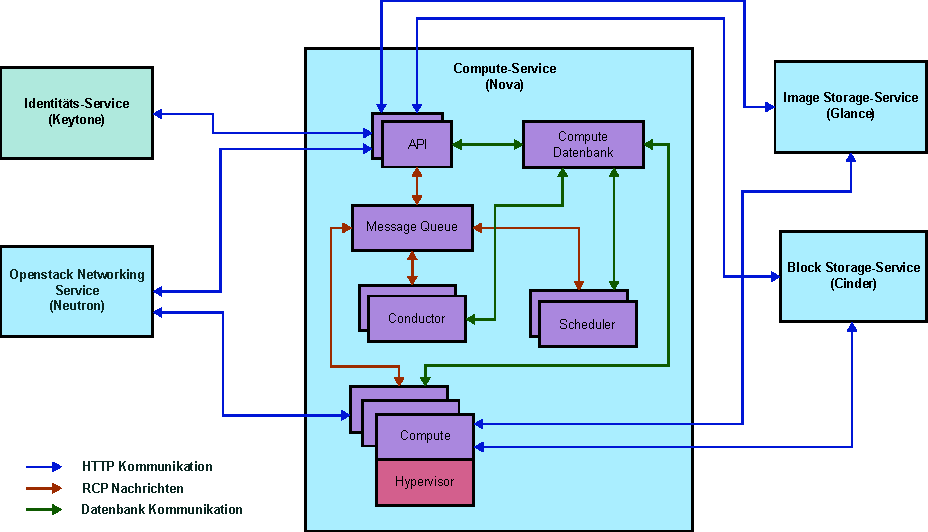
\includegraphics[width=\textwidth]{./content/graphics/compute_arch.pdf}
	\caption{Schematische Darstellung der OpenStack Compute Architektur}
	\label{compute_arch}
\end{figure}

Das Compute Modul interagiert mit den Hypervisoren durch einen API Server. Es unterstützt verschiedene Hypervisor implementierungen, die in der Cloud auch gemischt verwendet werden können. Das Compute Modul wird allerdings bei der Entwicklung hauptsächlich mit Kernelbasierter virtuellen Maschine (KVM) getestet, die ein Modul des Linux Kernels ist. 

Google Compute Engine

Microsoft Azure Logic Apps

VMware vRealize Suite

Amazon Web Services

OpenStack



\subsection{Container Orchestrierung}

Container Orchestrierung übernimmt die automatische Platzierung, Skalierung und Management von containerisierte Applikationen. Das Konzept ist dabei ähnlich wie bei der Orchestrierung von virtuellen Maschinen. Eine zentrale Orchestrierungsinstazn verwaltet mehrere Container Runtimes die oft auf verschiedenen physikalischen Maschinen laufen.

Eine der meistverbreiteten Implementierungen von Container Orchestrierungstools ist Kubernetes. Es kann entweder direkt auf dem Host Betriebssystem verwendet werden als Virtualisierungsmethode, oder auch in Kombination mit Cloud System Management verwendet werden um Applikationen auf den virtuellen Maschinen zu verwalten. Anhand der Funktionsweise und Architektur von Kubernetes wird im folgenden Abschnitt beispielhaft gezeigt, wie Tools für Container Orchestrierung umgesetzt werden können. Dieser ist in der Abbildung \ref{kubernetes_arch} dargestellt.

\begin{figure}[htbp]
	\centering
	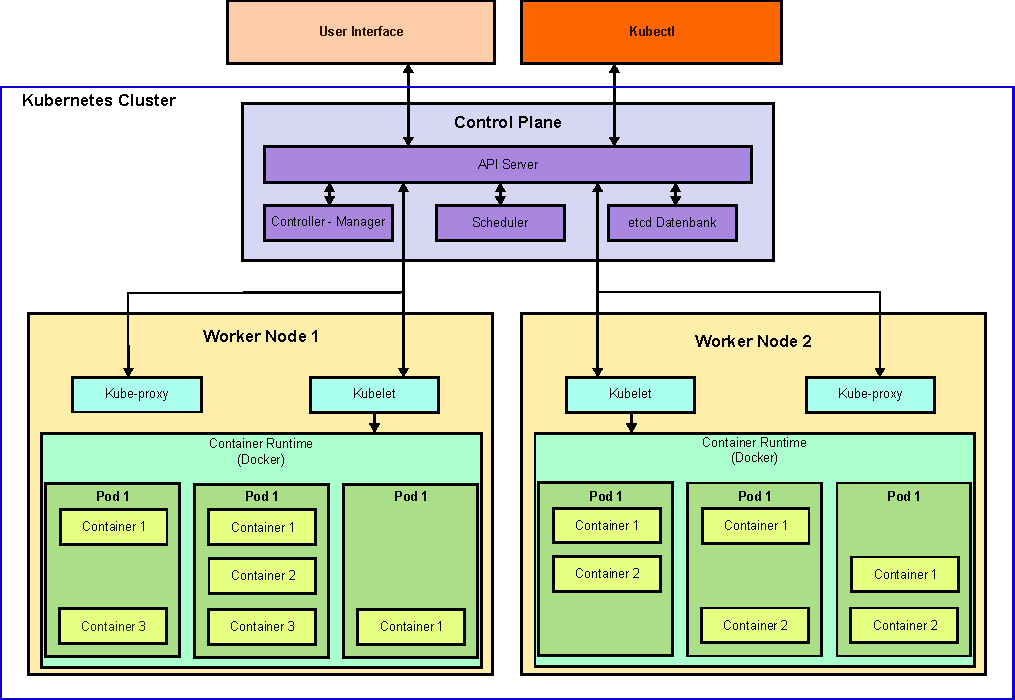
\includegraphics[width=\textwidth]{./content/graphics/kubernetes_arch.pdf}
	\caption{Schematische Darstellung der Kubernetes Cluster Architektur}
	\label{kubernetes_arch}
\end{figure}

Die containerisierte Applikationen werden bei Kubernetes in Pods gelegt, die auf den sogenannten \enquote{Worker Nodes} ausgeführt werden. Diese Nodes können sowohl auf virtuellen Maschinen als auch auf physikalischen Maschinen ausgeführt werden. Ein Node besteht aus mehreren Komponenten:

\begin{itemize}
	\item kubelet: Diese Komponente verwaltet die Container die in den Pods laufen. Hierfür werden PodSpecs Konfigurationen verwendet, die die Sollzustände der Container beschreiben in dem jeweiligen Pod beschreiben.
	\item kube-proxy: verwaltet die Netzwerkregeln auf den Nodes. Diese Regeln gelten für die Netzwerkkommunikation zu den Pods aus dem Netzwerk. 
	\item container runtime: Container Runtimes implementieren die Erstellung und Verwaltung von Container auf dem Betriebssystem. Kubernetes unterstützt verschiedene container Runtimes, am häufigsten wird Docker/Containerd verwendet. 
\end{itemize}

Die \enquote{Worker Nodes} werden von der \enquote{Control Plane} verwaltet. Diese besteht ebenfalls aus mehreren Komponenten, die die globale Entscheidungen über das Cluster treffen. Hierzu gehört die Verteilung der Container aber auch die Überwachung und das reagieren auf Ereignisse. Die einzelnen Komponenten können auch verteilt auf verschiedene Maschinen ausgeführt werden, in kleineren CLustern werden typischerweise alle Control Plane Komponenten auf derselben Maschine ausgeführt, die keine Worker Nodes ausführt. In größeren Produktionsumgebungen werden die Komponenten über mehrere Systeme verteilt ausgeführt. Die Control Plane besteht aus den folgenden Komponenten:

\begin{itemize}
	\item API Server: Der API Server stellt die API Schnittstelle für Kubernetes zur Verfügung. Es ist sowohl für die Kommunikation zwischen Benutzer und Kubernetes Cluster als auch für die Kubernetes Komponenten untereinander innerhalb des Clusters zuständig. 
	\item etcd Datenbank: Datenbank für alle Cluster Daten. Es ist nach dem Key-Value Storage 
	%\glsadd{Key-Value Storage}% 
	Prinzip implementiert. Änderungen erzeugen immer eine neue Version, 
	\item kube-scheduler: Diese Komponente erkennt neue Pods im System, die auf keinem Worker Node ausgeführt werden und wählt geeignete Nodes für sie aus, wo sie ausgeführt werden können. Die Auswahl an geeignete Worker Nodes wird an verschiedenen Kriterien festgelegt: individuelle und kollektive Ressourcenanforderungen, Hardware-/Software-/Richtlinienbeschränkungen, Affinitäts- und Anti-Affinitäts-Spezifikationen, Datenlokalität, Beeinträchtigung zwischen Workloads und Fristen.
	\item kube-controller-manager: Komponente der Control Plane, die Controller-Prozesse ausführt.
	
	Jede Art von Controller ist logisch ein separater Prozess, jedoch sind sie alle in einem Binärdatei Kompiliert und laufen in einem einzigen Prozess.
	
	Es gibt viele verschiedene Arten von Controllern. Einige Beispiele sind:

    Node Controller: Verantwortlich für das Erkennen und Reagieren, wenn Knoten ausfallen.
    Job Controller: Überwacht Job-Objekte, die einmalige Aufgaben darstellen, und erstellt Pods, um diese Aufgaben zu erfüllen.
    EndpointSlice Controller: Füllt EndpointSlice-Objekte aus (um eine Verbindung zwischen Services und Pods herzustellen).
    ServiceAccount Controller: Erstellt Standard-ServiceAccounts für neue Namespaces.

	Die obige Liste ist nicht vollständig.
\end{itemize}

Neue Worker Nodes im Kubernetes Cluster müssen im Control Plane registriert werden bevor sie Pods ausführen können. Dies erfolgt über den API Server. In der Standardkonfiguration registrieren sich Nodes selbständig, eine manuelle Registrierung ist ebenfalls möglich. Wenn alle nötigen Softwarekomponenten des Nodes laufen, wird es als Gesund deklariert und kann Pods ausführen. Identifikation der Nodes erfolgt über den Namen. Der Name darf aus diesem Grund nur einmalig im Cluster vorhanden sein. 

Die Verfügbarkeit von Nodes wird durch \enquote{Heartbeat} Nachrichten sichergestellt. Diese Nachrichten werden periodisch an die Control Plane gesendet, damit der aktuelle Node Status aktualisiert werden kann und ein nicht mehr verfügbarer Node erkannt werden kann. 

Innerhalb der Control Plane verwaltet die Node Controller Komponente des Controller Managers die verschiedenen Aspekte der Knoten. Sie erstellt eine Liste der im Cluster verfügbaren Knoten und deren Status. Sie weist den Knoten, falls diese Einstellung aktiviert ist, einen \gls{CIDR} Block zu und übernimmt somit die Verwaltung der Netzwerkkonfiguration im Cluster. Wenn Kubernetes im Cloud Management System verwendet wird, wird die Liste der Nodes mit der Liste der verfügbaren virtuellen Maschinen des Cloud Systems synchron gehalten. Ist ein Node nicht verfügbar, kommuniziert der Node Controller mit dem Cloud Management System und prüft, ob die virtuelle Maschine für den Node noch verfügbar ist. Ist dies nicht der Fall, wird der Node gelöscht. Die Nodes werden ebenfalls auf ihre korrekte Funktionalität überwacht, wenn ein Node nicht unerreichbar ist, werden Pods, die auf dem Node laufen sollten auf andere Nodes umgelagert. 

Die verfügbaren Rechenressourcen der jeweiligen Nodes wird bei der Registrierung übertragen. Dies beinhaltet beispielweise die verfügbare menge an Arbeitsspeicher und die Anzahl an CPU Kerne. Bei der automatischen Registrierung der Nodes passiert dies automatisch, wenn ein Node manuell hinzugefügt wird, müssen diese Informationen dabei angegeben werden. 

\section{Hardware und Softwareumgebung in Fahrzeugen}

Die zunehmende Automatisierung der Fahrfunktionen hat erhebliche Änderungen bei der verwendeten Hardware und Software in Fahrzeugen hervorgerufen. Die Zunahme an Sensoren und Rechenleistung hat zu neuen Hardware und Softwarearchitekturen geführt, die bisher hauptsächlich in IT Infrastrukturen üblich waren. 

\subsection{Hardwareumgebung in Fahrzeugen}

Traditionell wurden elektrische Komponenten in Fahrzeugen dezentralisiert entwickelt. In diesem Ansatz sind einzelne Steuergeräte mit deren Software möglichst alleinig für bestimmte Funktionalitäten verantwortlich, die Kopplung zwischen den einzelnen Steuergeräten ist möglichst lose gestaltet, die über Bussysteme untereinander Daten austauschen können. Dies ermöglicht eine einfache Separation von Zuständigkeiten und eine simple Verifikation der Integrationsvoraussetzungen. \cite{DiNatale2010} Dieser Ansatz bietet eine höhere Kontrolle über die einzelnen Systeme und eine hohe Flexibilität für verschiedene Varianten. Nachteilig ist, dass wenn implementierte Funktionen nicht mehr auf einzelne Steuergeräte beschränkt werden können, ein Overhead aufgrund der nötigen Kommunikation zwischen Steuergeräte entsteht. Dies führt einerseits zu hohe Auslastungen auf den Kommunikationsbussen und einem erhöhten Aufwand bei der Abstimmung der Kommunikationsschnittstellen. \cite{Reinhardt2013} Die dezentralisierte Architektur hat sich in den 1980-er Jahren etabliert, durch die Zunahme an automatisierte Fahrfunktionen und Komfortfunktionen stieg die Anzahl an Steuergeräte in modernen Fahrzeugen auf über 100 Stück. \cite{Amend2017} Insgesamt führt diese Architektur zu höheren Kosten aufgrund der hohen Anzahl an Steuergeräten und benötigte Busbandbreite. Aus diesem Grund entwickelt sich die E/E Architektur von modernen Fahrzeugen Richtung zentralisierte Architektur. 

Der erste Entwicklungsschritt nach der dezentralisierten Architektur ist die Domänenarchitektur. Fahrzeugdomänen sind Gruppen von Systemen und Funktionen, die einem bestimmten Entwicklungsbereich zugeordnet werden können. Diese sind beispielweise Antriebsstrang, Bremssystem, Chassis, Elektronik, Mensch-Maschine Schnittstellen. \cite{continental2024} Bei dieser Architektur sind Steuergeräte der gleichen Domäne miteinander vernetzt. Zusätzlich bekommt jede Domäne ein Domänensteuergerät, das als Master Steuergerät Funktionalitäten von mehreren herkömmlichen Steuergeräten vereint. Kommunikation zwischen Domänen ist durch eine Gateway Komponente möglich, die Nachrichten zwischen den verschiedenen Bussen überträgt. Diese Architektur ist in modernen Fahrzeugen sehr verbreitet. Durch fortschreiten der autonomen Fahrfunktionen und Infotainment Funktionalitäten ist diese Architektur mittlerweile auch nicht mehr Effizient, da die Abgrenzung der Funktionen auf einzelne Domänen nicht mehr möglich ist. Ein Abstandshalter Tempomat muss beispielweise sowohl Antriebsstrang als auch Bremse bedienen können. Für vollautonomes Fahren müssen weiterhin auch Lenkfunktionen, sowie mehrere Sensoren und Kameradaten kombiniert werden. Aus diesem Grund ist die Aufteilung der E/E Architektur auf Fahrzeugdomänen für zukünftige Fahrzeuge nicht mehr Zielführend. 

Die Zonenarchitektur teilt die Implementierte Funktionalitäten der Steuergeräte nicht nach Fahrzeugdomäne ein, sondern nach örtliche Anordnung im Fahrzeug. \cite{Chou2023} Diese Zonencontroller übernehmen Domänenübergreifende Funktionen und reduzieren die Anzahl an Busverbindungen und Steuergeräte. Ein zentrales Hochleistungssteuergerät übernimmt die Koordination der Kommunikation zwischen den Zonen sowie Funktionalitäten, die Zonenübergreifend sind. Hierzu gehören beispielweise Autonome Fahrfunktionen. In dieser Ansatz wird also die Anzahl an Steuergeräte weiter reduziert indem die einzelnen Steuergeräte leistungsstärker sind und mehr Funktionen implementieren. 

Die zentrale Architektur ist ein Konzept, welches die Funktionsbereiche der Zonensteuergeräte ebenfalls in das zentralen Steuergerät verlagert. Hierdurch wird die Anzahl an Steuergeräte auf ein Minimum reduziert. Eine Übersicht der vorgestellten Architekturen in Fahrzeugen bietet die Abbildung \ref{E/E_arch}.

\begin{figure}[htbp]
	\centering
	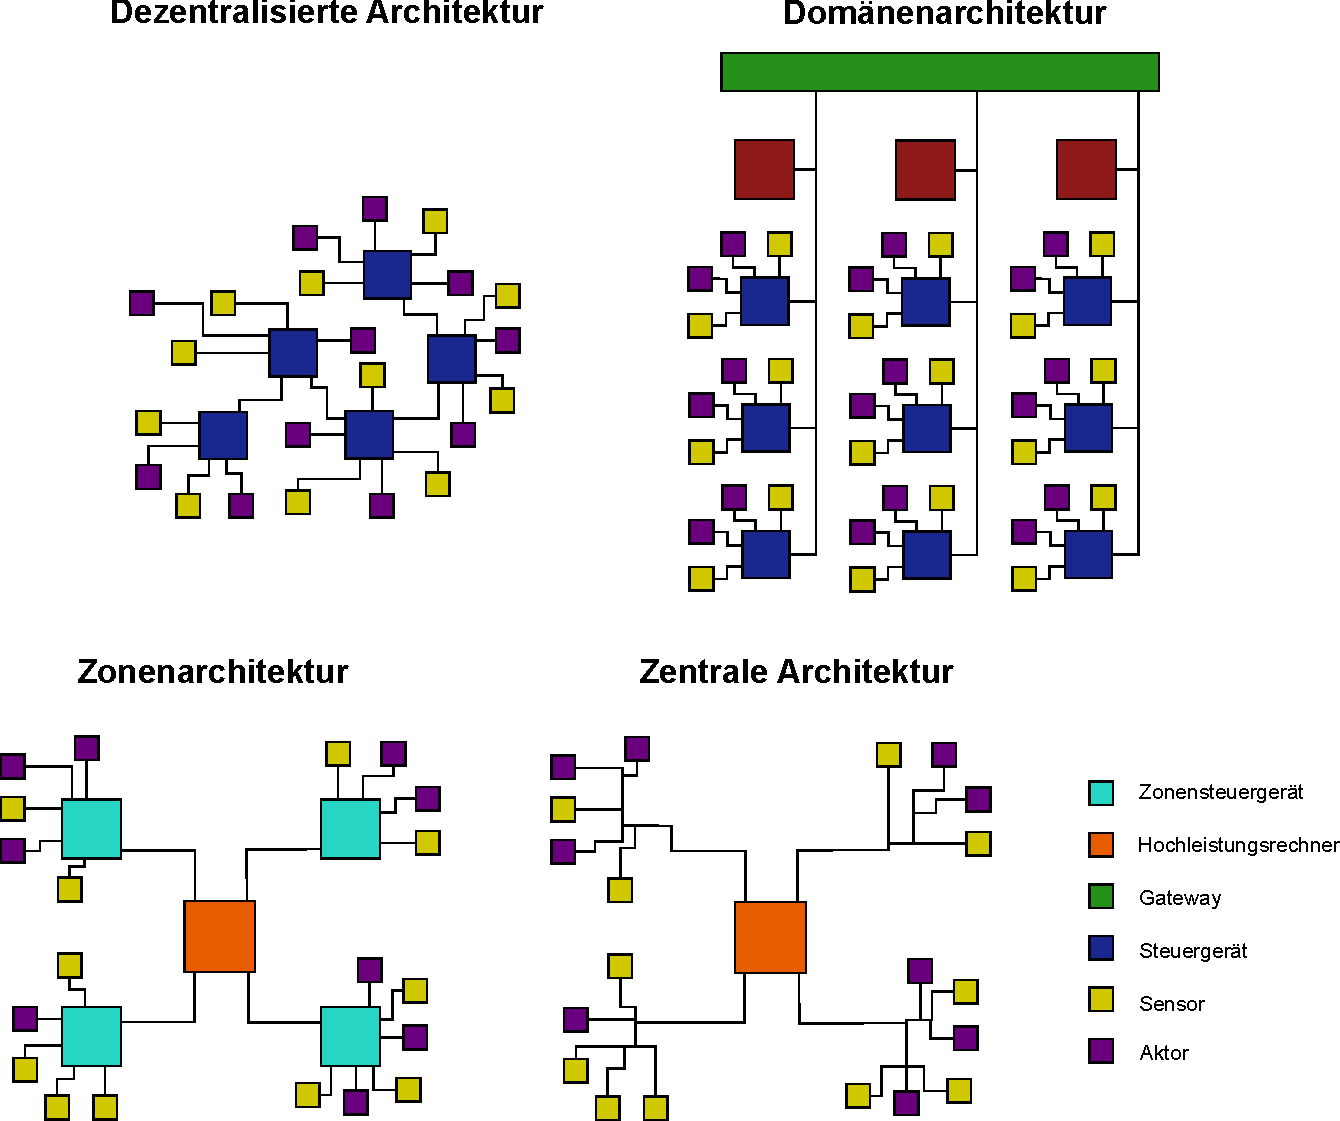
\includegraphics[width=\textwidth]{./content/graphics/EE_arch.pdf}
	\caption{Überblick über die E/E Architekturen in Fahrzeugen}
	\label{E/E_arch}
\end{figure}

Sowohl durch die Zentralisierung der Funktionalitäten als auch durch die technische Entwicklung im Bereich Fahrfunktionen und Infotainment steigt die benötigte Rechenleistung für die Steuergeräte. Im dezentralisierten Ansatz werden Steuergeräte verwendet die auf ihre Funktion spezialisiert sind. Sie benötigen nur begrenzt hohe Rechenleistung und eine begrenzte Anzahl an Interfaces um ihre Funktion zu erfüllen. 

Zonensteuergeräte, die im Zonenarchitektur zur Verwendung kommen, haben drei hauptrollen:
	\begin{itemize}
		\item Gateway: Implementiert eine Kommunikationsschnittstelle zwischen den Bussen der jeweiligen Zone und das Zentralsteuergerät.  Zudem interpretiert und verteilt es Befehle vom zentralen Fahrzeugcomputer an lokale Steuergeräte und Aktoren. Das Steuergerät ist is also auch für die Kommunikationssicherheit und lokale Netzwerküberwachung zuständig. 
		\item Aktuator: Konzeptabhängig implementiert das Zonensteuergerät zonenspezifische Funktionen wie Karosserieaktuation, Batteriemanagement, LED-Steuerung, Motorsteuerung oder andere Fahrwerks- und Antriebsfunktionen, die sicherheitskritisch sein können. 
		\item Spannungsversorgung: Das Zonensteuergerät agiert als intelligente Leistungsverteileinheit um die Zonenkomponenten mit Spannung zu versorgen und deren Leistungsverbrauch zu überwachen. 
	\end{itemize} \cite{Heurtefeux2021}

Zonensteuergeräte müssen die Konnektivität zu Busverbindungen zur Verfügung stellen, präzise Zeitsynchronisation ermöglichen und Nachrichten mit niedrige Latenzen umleiten können (innerhalb von wenigen Mikrosekunden). Für die Aktuator und Leistungsverteileinheit Funktionen muss das Steuergerät die entsprechenden Schnittstellen zur Verfügung stellen wie \glsxtrshort{PWM}, \glsxtrshort{SPI}, \glsxtrshort{UART}, \glsxtrshort{GPIO} und \glsxtrshort{ADC}-s. Ein Ansatz besteht darin hierfür generische Steuergeräte zu entwickeln, die flexibel für verschiedene Fahrzeuge eingesetzt werden können.\cite{Maier2023}

Zentralsteuergeräte sind sowohl in der Domänenarchitektur als auch in der Zentralen Architektur vorhanden. Sie übernehmen rechenintensive, Zonenübergreifende Funktionen wie zum Beispiel autonome Fahrfunktionen. Aus diesem Grund benötigen diese Steuergeräte eine deutlich höhere Rechenleistung als es in dezentralisierten Ansätzen üblich war. Für diese höhere Anforderungen werden \glsxtrshort{SoC}-s verwendet. Als Beispiel kann das FSD Steuergerät von Tesla betrachtet werden. 

Das Steuergerät nutzt zwei separate FSD Chips, die unabhängig voneinander jeweils ihr eigenes Betriebssystem ausführen. Die beiden Chips sind redundant ausgelegt für maximale Sicherheit, besitzen eigene Spannungsversorgungen und eigene Sensoren. Der FSD Chip ist ein \glsxtrshort{SoC} und beinhaltet folgende Hauptkomponenten:

\begin{itemize}
	\item 12 CPUs der Typ A72
	\item GPU der Typ G71
	\item 2 Neural Network Accelerator
	\item ISP und Video Encoding
\end{itemize}

Die Algorithmen für die autonome Fahrfunktionen werden auf den CPU Kernen ausgeführt. Neue Eingangsdaten werden zuerst vom Signalprozessor verarbeitet und anschließend im Speicher abgelegt. Wenn neue Daten verfügbar sind, überreicht die CPU die Daten an den Neural Network Accelerator. Sobald die Ausgangsdaten verfügbar sind, führt die CPU die entsprechenden Algorithmen aus. \cite{Talpes2020}

Zentralsteuergeräte implementieren viele gängige Architekturansätze aus der Informationstechnik um die benötigte Rechenleistung zu erreichen. Die verwendeten Mikroprozessoren besitzen mehrere Rechenkerne, es wird eine GPU für höhere Grafikleistung verwendet sowie andere spezifische Recheneinheiten verwendet, wie für das Ausführen von neuronalen Netzen. Diese einzelnen Komponenten werden meistens als \glsxtrshort{SoC} in einem Chip kombiniert.

\subsection{Softwareumgebung in Fahrzeugen}

Sowohl die gestiegene Funktionsumfang, Komplexität und Bedarf an Aktualisierbarkeit der Softwarefunktionen als auch die hierdurch eingeleitete Zentralisierung der \glsxtrshort{E/E} Architektur und damit verbundene gestiegene Rechenleistung und Komplexität der Steuergeräte stellen neue Anforderungen an die verwendeten Software in den Steuergeräten. 

Bei der dezentralisierten \glsxtrshort{E/E} Architektur ist die Software in den meisten Fällen monolithisch ausgelegt. Es findet entweder keine Aktualisierung im Lebenszyklus des Fahrzeugs statt, oder es wird das gesamte Steuergerät oder Software ausgetauscht. Die Geschwindigkeit,  mit der Innovationen im Bereich Software und Hardware im Automobilbereich voranschreiten hat in den letzten Jahren stark zugenommen. Die Entwicklungszyklen für Softwarekomponenten sind mittlerweile deutlich kürzer als der Lebenszyklus der Fahrzeuge, Aktualisierbarkeit der Software muss also für die zukünftige Architekturen eine wichtige Rolle spielen. \cite{Mundhenk2017} 

Für die leistungsstärkere Domänen- und Zentralsteuergeräte werden CPUs mit mehreren Kernen eingesetzt. Software, die für Einzelkernprozessoren implementiert wurde, muss entweder auf einem Kern portiert werden oder neu implementiert werden, so dass es als Prozess oder mehrere Prozesse auf einem oder mehreren Kernen ausgeführt werden kann. \cite{Widlund2017} Die Funktionalitäten der einzelnen Steuergeräte werden also von sogenannten Software-definierten-Funktionen ersetzt, die einfach ausgerollt, und ausgetauscht werden können. Dieser Ansatz benötigt ein geeignetes Betriebssystem. Steuergeräte, die in der dezentralisierten Architektur verwendet werden und nur eine eine sehr eingeschränkte Anzahl an Funktionalitäten implementieren verwenden entweder kein Betriebssystem oder ein \glsxtrshort{RTOS}. \glsxtrshort{RTOS} ist ein Betriebssystem, welches auf die Einhaltung von Ausführungszeiten und Reaktionszeiten optimiert ist, und somit Echtzeitfähigkeit garantiert. Domänen- und Zentralsteuergeräte benutzen Hardwarekomponenten aus dem \glsxtrshort{PC} Bereich, für diese Hardwareplattforme sind Betriebssysteme geeignet, die ebenfalls im \glsxtrshort{PC} Bereich verwendet werden, da sie eine Laufzeitumgebung bieten, die bereits Treiber und Software Bibliotheken beinhaltet um die Hardware optimal auszunutzen. Mehrere Automobilhersteller setzen bereits auf dem Open Source Betriebssystem Linux für deren leistungsfähige Steuergeräte: BMW \cite{Foss2019}, Tesla \cite{Tesla2024} und Toyota \cite{endgadget2017} verwenden jeweils ein entsprechend angepasstes Linux Betriebssystem.

Wie ein Betriebssystem für ein Hochleistungssteuergerät implementiert werden kann, wird anhand des Betriebssystems \enquote{DriveOS} vorgestellt. DriveOS wird von Nvidia entwickelt und bereitgestellt und ist für die Verwendung auf Steuergeräte für autonome Fahrzeuge konzipiert, die Nvidia Hardware verwenden. \cite{Nvidia2024} DriveOS nutzt Virtualisierung um mehrere Betriebssysteme auszuführen. Um sowohl die Echtzeitfähigkeit von \glsxtrshort{RTOS} als auch die Kompatibilität von PC Betriebssystemen zu kombinieren führt DriveOS ein \glsxtrshort{RTOS} namens Quest aus, welches gleichzeitig Hypervisor Funktionalitäten besitzt um weitere Betriebssysteme zu starten. Diese weitere Betriebssysteme können Linux Systeme sein. Durch dieses Konzept können Funktionen, die Echtzeitfähigkeit erfordern im \glsxtrshort{RTOS} System platziert werden, nicht Zeitkritische Anwendungen können im Linux System mit weniger Aufwand integriert werden. Kommunikation zwischen den Betriebssystemen wird durch einen geteilten Speicherbereich ermöglicht. 
\cite{Sinha2021}

Durch die erhöhte Komplexität der Softwarefunktionen und die erhöhte Rechenleistung in den Steuergeräten werden Technologien, die in der \glsxtrshort{IT} Infrastruktur verwendet werden auch in Fahrzeugen integriert. Betriebssysteme, Software Bibliotheken, Virtualisierungstechnologien sind Beispiele hierfür, die mittlerweile auch in Fahrzeugen verwendet werden.

\section{Verteiltes Rechnen in Fahrzeugen}




